\chapter{Feature Selection}
\label{ch:feature-selection}
\index{Feature Selection|(}

\textit{Feature Selection} (FS) is a process that chooses an optimal subset of features according to certain criterion \citep{liu2012feature}. According to \citet{sammut2017encyclopedia}, in many real-world applications such as: data mining, machine learning, computer vision, and bioinformatics we need to deal with high-dimensional data. Lately, the dimensionality of the data involved in these areas has increased exponentially. The trend of this growth is also reflected in the \textit{UCI machine learning repository}\footnote{https://archive.ics.uci.edu/ml/index.php} as shown in Figure~\ref{fig:fs_growth}.

\begin{marginfigure}
  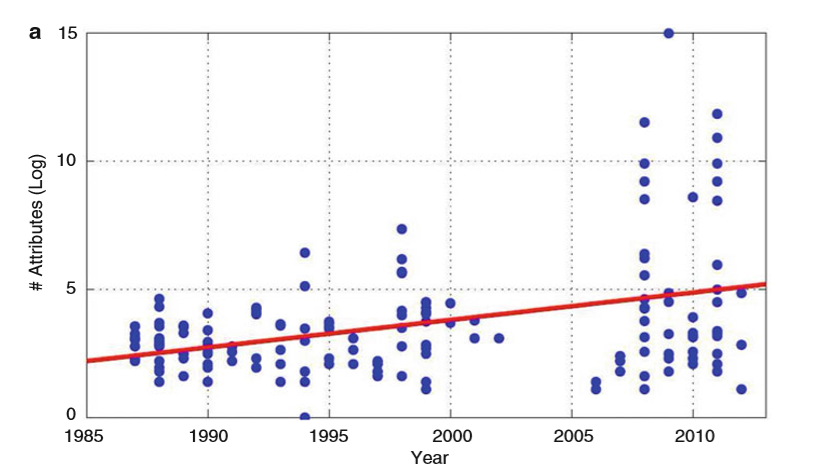
\includegraphics{feature_selection/growth.png}
  \caption{Growth of the number of features in the UCI ML repository. Reproduced from \citet{sammut2017encyclopedia}.}
  \label{fig:fs_growth}
\end{marginfigure}

\citet{guyon2003introduction} state that the objective of FS is three-fold: improving the prediction performance of the predictors, providing faster and more cost-effective predictors, and providing a better understanding of the underlying process that generated the data. Furthermore, the aim of the FS is to select features that are \textit{independent} of each other but \textit{highly dependent} on the value to be predicted.

FS keeps the original feature, that is, it maintains the physical meanings of the original feature without any transformation. Furthermore, \citet{masaeli2010transformation} found that this property has its significance in many practical applications such as finding relevant genes to a specific disease and building a sentiment lexicon for sentiment analysis.

According to \citet{zhao2010advancing}, FS is an optimization problem that can be split into two perspectives:
\begin{enumerate}
  \item searching for the best subset of features,
  \item principle model for: selecting, adding, removing or changing new features during the search using a certain evaluation measure.
\end{enumerate}
Mainly there are three models used for FS: filter, wrapper and embedded.

\section{Filter models}\label{sec:fs_filter}\index{Feature Selection!Filter models}
\textit{Filter models} operate independently of the learning algorithm. A filter algorithm usually consists of two steps. First, each feature is given a weight then, the features are ranked and the top-ranking features are chosen whilst the others are discarded. \nameref{sec:fs_criteria} section describes some popular measurements used to calculate feature weight.

\subsection{Selection criteria}\label{sec:fs_criteria}
\begin{itemize}
  \item \textit{Correlation}\index{Feature Selection!correlation}: this measures the ability to predict the value of one variable from the value of another. In FS for classification, we look for how strongly a feature is associated with the class. A feature $x_{1}$ is preferred to another feature $x_{2}$ if the association between feature $x_{1}$ and class $Y$ is higher than the association between $x_{2}$ and $Y$. In FS for clustering, the association between two random features measures the similarity between the two \citep{liu2005toward}. According to \citet{guyon2003introduction}, one of the simplest dependency measure function is \textit{Pearson's correlation coefficient} defined in Eq.~\ref{fs_pearson}, where $x_{i}$ is the $i_{th}$ feature, $Y$ is the output (class labels), $cov$ is the covariance and $var$ is the variance.
  \begin{equation}\label{fs_pearson}
    \rho(i) = \frac{cov(x_{i},Y)}{\sqrt{var(x_{i})*var(Y)}}
  \end{equation}
  \item \textit{Information gain}\index{Feature Selection!information gain}:  this is one of the most popular measures in FS due to its computational efficiency and simple interpretation \citep{tang2014feature}. It is used to measure the dependence between features and labels. The information contained in label $Y$ can be defined by \textit{Shannon's entropy} $H(Y)$. This is defined in Eq.~\ref{fs_entropy1} where $y_{j}$ are the labels and $P(y_{j})$ is their probability. If we observe feature $X$ then the conditional entropy $H(Y, X)$, can be defined by Eq.~\ref{fs_entropy2} where $P(y_{j},x_{i})$ is the joint probability. Finally, \textit{mutual information} $MI(Y,X)$ between label $Y$ and feature $X$ can be defined by Eq.~\ref{fs_mi}.
  \begin{equation}\label{fs_entropy1}
    H(Y) = -\sum_j P(y_{j})\log_{2} P(y_{})
  \end{equation}  
  \begin{equation}\label{fs_entropy2}
    H(Y, X) = -\sum_i\sum_j P(y_{j},x_{i})\log_{2}P(y_{j},x_{i})
  \end{equation}
  \begin{equation}\label{fs_mi}
    MI(Y,X) = H(Y) - H(Y|X)
  \end{equation}
  %\item \textit{Consistency measure}\index{Feature Selection!consistency measure}: this type of evaluation measure is characteristically different from other measures because of it's heavy reliance on the training dataset and use of Min-Features bias in selecting a subset of features. Min-Features bias prefers consistent hypotheses definable over as few features as possible. This measure finds out the minimal size subset that satisfies the acceptable inconsistency rate, that is usually set by the user \citep{liu2005toward}.
\end{itemize}

Filter models normally are very fast because usually the evaluation measurement complexity is simple and cheap, both in terms of performance and memory. Having said this, \citet{garcia2015data} found that due to it's simplicity and low time complexity it can handle large data. On the other hand, \citet{guyon2003introduction} found that due to the fact that filter models score features independently of each other, the best features are not always chosen. This is because, a feature that is completely useless by itself thus ranked very low with this model, can provide a significant performance improvement when taken with others. \textit{Wrapper models} address this limitation by evaluating subsets of features rather than individual features.

\section{Wrapper models}\label{sec:fs_wrapper}\index{Feature Selection!Wrapper models}
The aim of the \textit{Wrapper model} is to achieve the highest predictive accuracy possible by selecting the features that accomplish this for a fixed learning algorithm. It uses a learning algorithm as a black-box to select the best feature subset, agreeing on a predictive measure \citep{kohavi1995study}. Figure~\ref{fig:fs_wrapper} shows a conceptual view of a wrapper model. The \textit{Feature Selector} component takes on the original features and uses a search strategy to generate subsets of features for evaluation. The selected feature subset uses the learning algorithm to \textit{measure} and evaluate its performance. These steps are repeated until a \textit{stopping criterion} is met. Typically, the stopping criterion is that refinements to the subset do not yield any performance improvements.

\begin{figure}
  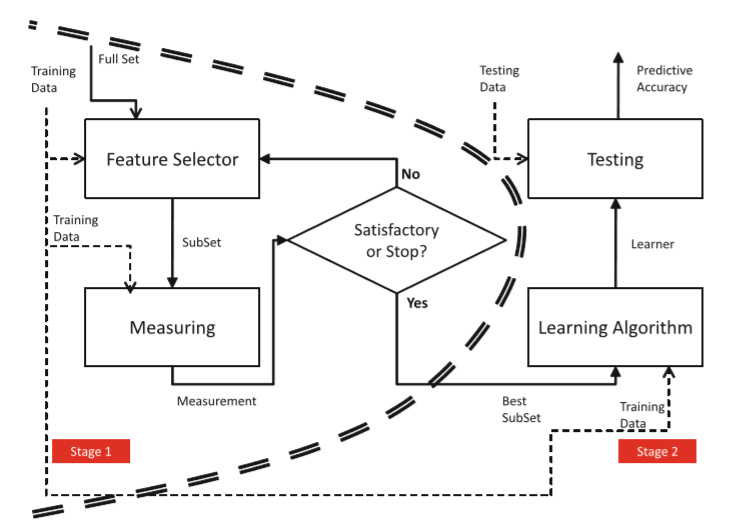
\includegraphics{feature_selection/wrapper.png}
  \caption{A general framework for Wrapper Methods of FS. Reproduced from \citet{tang2014feature}}
  \label{fig:fs_wrapper}
\end{figure}

\textit{Feature Selector} plays an important role in wrapper models because the order of the feature search space is $O(2^N)$ (Figure~\ref{fig:fs_search_space}) making exhaustive search methods computationally unfeasible for large datasets. Therefore, search algorithms such as \textit{Sequential selection algorithms} and \textit{Heuristic selection algorithms}, described in section \nameref{sec:fs_search_algo}, need to be used \citep{chandrashekar2014survey}.

\begin{marginfigure}
  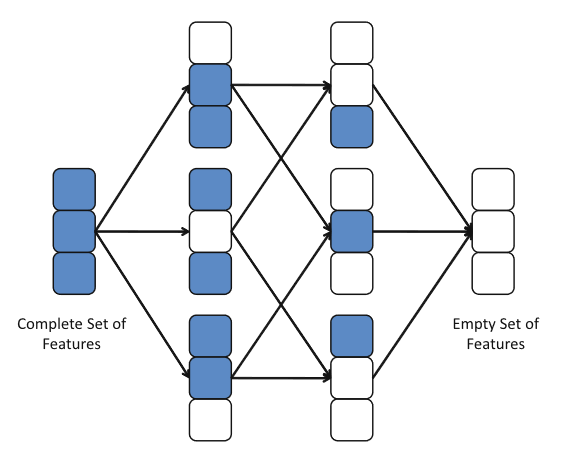
\includegraphics{feature_selection/search_space.png}
  \caption{Search space for FS. Reproduced from \citet{liu2012feature}}
  \label{fig:fs_search_space}
\end{marginfigure}

\subsection{Search algorithms}\label{sec:fs_search_algo}
\begin{itemize}
  \item\textbf{Sequential selection algorithms}\index{Feature Selection!Sequential selection algorithms}: These algorithms are called sequential due to the iterative nature of the algorithms. Sequential forward feature selection (SFFS), sequential backward feature elimination (SBFE) and sequential bidirectional selection are greedy search algorithms that add or remove features one at a time \citep{liu2005toward}. SFFS initiates with an empty set and SBFE initiates with a full set where as a bidirectional search initiates a SFFS and SBFE simultaneously ensuring that the features selected by SFFS are never eliminated by SBFE. The mentioned algorithms suffer from producing nested subsets since the forward inclusion is always unconditional which means that two highly correlated variables might be included if it gave the highest performance in the SFFS evaluation \citep{chandrashekar2014survey}. \citet{sun2006comparison} developed the Adaptive Sequential Forward Floating Selection (ASFFS) algorithm, an adaptive version of the SFFS, to avoid the nesting effect and produce a less redundant subset than the SFFS algorithm.
  \item\textbf{Heuristic algorithms}\index{Feature Selection!Heuristic algorithms}: One of the widely used \textit{Heuristic algorithm} in FS is \textit{Genetic algorithm} (GA); a general adaptive optimization search methodology that mimic Darwinian forces of natural selection to find optimal values of some function \citep{chandrashekar2014survey}. The algorithm starts by creating a set of candidate solutions referred to as chromosomes which form the first population. For each chromosome the fitness value is calculated. The fitness value is randomly impacted mainly by the \textit{crossover} and \textit{mutation} functions. Then based on the Darwinian principle of 'survival of the fittest' referred to \textit{offspring}, the chromosomes with the best fitness values are combined randomly to produce the next population. This process is repeated again until acceptable results are obtained. For FS, a simple GA approach is to encode features in the chromosome (e.g. the chromosome 01001000 could mean that the 2nd and 5th features are selected), and the fitness value can be some measurement of model performance \citep{de2015grammar}. \citet{huang2006ga} used a chromosome with parameters of a \textit{Support Vector Machines} SVM and the resultant solution provided the best features and the appropriate SVM parameters.
\end{itemize}

According to \citet{sammut2017encyclopedia}, wrapper models generally achieve better recognition rates than filter models since the learning algorithm is involved in the selection of the subset, thus any bias introduced by the chosen algorithm is removed. The drawback of this model is that, wrapper models must train a classifier for each feature subset thus the method might become unfeasible.

\section{Embedded models}\label{sec:fs_embedded}\index{Feature Selection!Embedded models}
Some learning algorithms have in-built mechanisms to deal with feature selection \citep{guyon2003introduction,sammut2017encyclopedia}. This makes the selection of the features more efficient than the wrapper method and is specifically designed for the algorithm of choice. Another improvement on the other methods is that whilst the filter and wrapper methods select the features as part of the pre-processing of the data, the embedded models cater for feature selection as part of the learning process. One such example is the use of \textit{L1-norm} regularisation in (SVM) \citep{guyon2003introduction,de2015grammar}. Here the coefficients of less important features are reduced to zeros thus eliminating them. \textit{L2-norm} regularisation can also be used for feature selection but was found to be less effective than \textit{l1-norm} regularisation \citep{de2015grammar}. \textit{Decision trees} also have a feature selection strategy embedded within the algorithm \citep{garcia2015data}.

\index{Feature Selection|)}